
\newpage
\section{Appendix B}
\subsection{Reference \acl{mimp} sequences}
\begin{table}[h]
\caption{Reference \ac{mimp} sequences used to build \ac{hmm}}
\label{apx:RefMimps}
\resizebox{\columnwidth}{!}{%
\begin{tabular}{llcc}
\multicolumn{1}{c}{Isolate Source} & \multicolumn{1}{c}{Sequence Name} & Size (bp) & GenBank Accession \\
\textit{Fusarium oxysporum f. sp. lycopersici} & Fusarium oxysporum f. sp. lycopersici MITE mimp4, complete sequence & 220 & EU833101.1 \\
\textit{Fusarium oxysporum f. sp. melonis} & Fusarium oxysporum f. sp. melonis MITE mimp3, complete sequence & 216 & EU833100.1 \\
\textit{Fusarium oxysporum} & Fusarium oxysporum repetitive element mimp2 & 213 & AF076625.1 \\
\textit{Fusarium oxysporum} & Fusarium oxysporum repetitive element mimp1 & 223 & AF076624.1
\end{tabular}%
}
\end{table}

\newpage
\subsubsection{\Acl{tef} phylogeny and \acl{cec} distribution from \acl{Foa} and \acl{Foci} isolates.}
\begin{sidewaysfigure}[hp!]
    \centering
    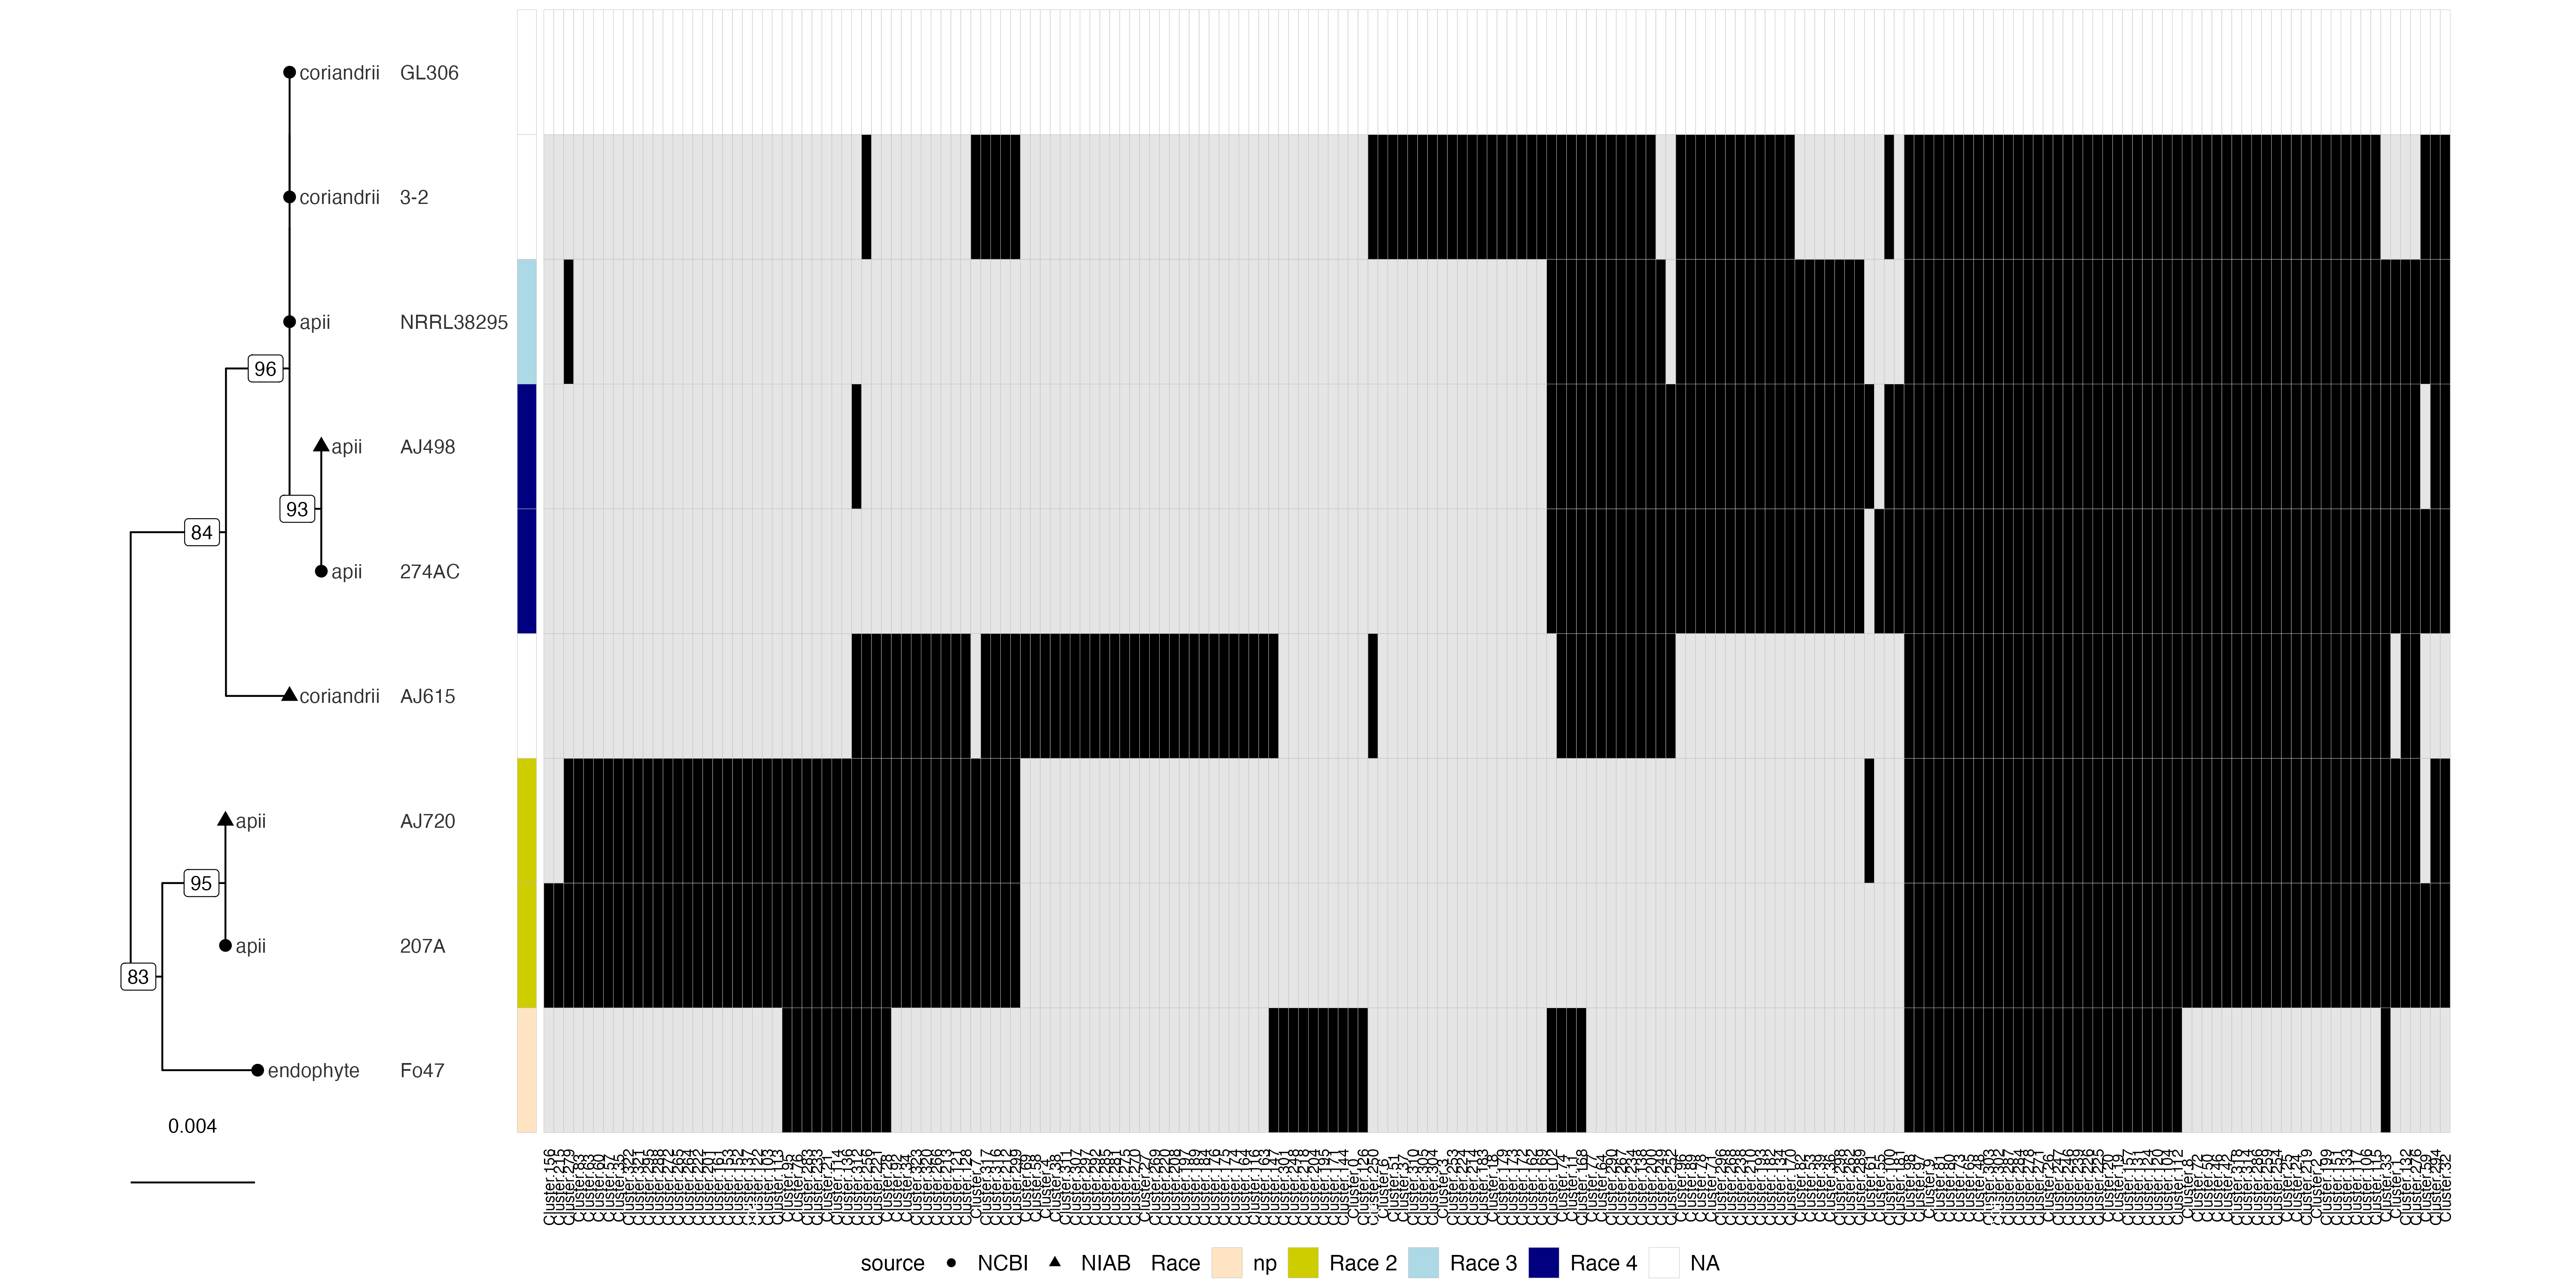
\includegraphics[width=0.8\textwidth]{Figures/HeatmapAndPhylo_ApiiAndCoriandriiOnly.png}
    \captionsetup{width=20cm}
    \caption[Maximum likelihood phylogeny from alignment of \Acl{tef} sequences from \acl{Foa} and \acl{Foci} isolates alongside respective \acl{cec} profiles.]{\textbf{Maximum likelihood phylogeny from alignment of \Acf{tef} sequences from \acf{Foa} and \acf{Foci} isolates alongside respective \acf{cec} profiles.} Branch length shows the expected number of substitutions per site. White boxes indicate bootstrap values from 1000 bootstrap replicates. IQ-TREE2 (v2.2.0.3) best model of substitution; TNe+G4. \Acfp{fsp} and isolate codes are indicated at tree tips. \Acp{cec} were determined using CD-HIT (v4.8.1) at 80\% identity, following \ac{ce} identification using TBLASTN, (cut-off 1e-6 65\% identity and coverage threshold) and filtering using SignalP (v5.0b) and EffectorP (v2.1.0). \ac{Fo} isolate Fo47 was included for \ac{cec} profile comparison against non-pathogen. np indicates non-pathogen. \ac{Foci} GL306 was not included in the \ac{Maei} analysis.}
    \label{fig:Maei_celeryandcoriander}
\end{sidewaysfigure}